%\documentclass{ut-thesis}
\documentclass{thesis}

%**************************** General libraries *******************************
\usepackage{mathtools,mathrsfs}
\usepackage{cancel}
\usepackage[utf8]{inputenc} 
\usepackage{amssymb}
\usepackage{ntheorem}
\usepackage{tensor}
%\usepackage{physics}
\usepackage[italicdiff]{physics}
\usepackage{calc}
\usepackage{caption}
%\usepackage{subcaption}
\usepackage{tcolorbox}
\usepackage{chngcntr}
\usepackage{titlesec}
\usepackage {graphicx,float} 
\usepackage{subfig}
\usepackage{siunitx}
\usepackage{xcolor}
\usepackage{etoolbox} %ifthen
\usepackage[outline]{contour} % glow around text
\usepackage{boondox-cal}

%**************************** Bibliography management *******************************
\usepackage{biblatex} %Imports biblatex package
\addbibresource{sample.bib} %Import the bibliography file



%**************************** Tikz libraries *******************************
\usepackage{tikz}
\usetikzlibrary{external}
\tikzexternalize[prefix=./Externalized_figures/]
%\tikzset{external/mode=graphics if exists}
%\tikzexternalize

\usepackage{tikz,pgfplots}
\usetikzlibrary{shapes,arrows,arrows.meta,spy}
\usetikzlibrary{calc}% needed for BB
\usepackage{pgfplots}
\usetikzlibrary{math} % for \tikzmath
\usetikzlibrary{angles,quotes} % for pic (angle labels)
\usetikzlibrary{decorations.pathmorphing,decorations.markings}
\usetikzlibrary{decorations.pathreplacing} % for curly braces
\usetikzlibrary {decorations.markings,shapes.arrows}
\usetikzlibrary{patterns}
\usepackage{tkz-euclide}
\usepackage{tikz-3dplot}
\usetikzlibrary{patterns,patterns.meta}
\usepgfplotslibrary{fillbetween}
\usetikzlibrary{patterns.meta}
\usepackage{physics}
\usepackage{tikz}
\usepackage{tikz-3dplot}
\usepackage[outline]{contour} % glow around text
\usepackage{xcolor}
\usepackage{tikz-3dplot-circleofsphere}
%\usetikzlibrary{3d,angles,quotes,calc}

%**************************** custom macro's *******************************
\newsavebox\CBox
\newcommand\hcancel[2][0.5pt]{%
  \ifmmode\sbox\CBox{$#2$}\else\sbox\CBox{#2}\fi%
  \makebox[0pt][l]{\usebox\CBox}%  
  \rule[0.5\ht\CBox-#1/2]{\wd\CBox}{#1}}
%\newcommand{\edal}{\end{align}}
%\newcommand{\bgal}{\begin{align}\end{align}}
\newcommand{\Lagr}{\mathcal{L}}
\newcommand{\questeq}{\overset{?}{=}}
%\newtheorem{theorem}{Theorem}
\newtheorem{lemma}{Lemma}
\renewcommand\thelemma{\unskip}
\newcommand{\christ}[3]{\ensuremath{\Gamma^{#1}_{#2#3}}}
\newcommand{\half}{\ensuremath{\frac{1}{2}}}
\newcommand{\kwart}{\ensuremath{\frac{1}{4}}}
\newcommand\del{\overline{\boldsymbol{{\triangledown}}}}
\newcommand\maal{\boldsymbol{\times}}
\newcommand\spatie{\quad\quad\quad\quad}
\newcommand\Breal{\mathbb{R}}
\newcommand\Qiuu{\mathbb{Q}}
\newcommand\Bint{\mathbb{Z}}
\newcommand\Bnat{\mathbb{N}}
\newcommand\Bcomp{\mathbb{C}}
\newcommand\Zed{\mathbb{Z}}
\newcommand\En{\mathbb{N}}
\newcommand\Pee{\mathbb{P}}
\newcommand\RZO{\mathbb{R}_{[0,1]}}
\newcommand\Et{\text{ and }}
\newcommand\Ou{\text{ or }}
\newcommand\Ieoi{\Leftrightarrow }
\newcommand\Iff{\Leftrightarrow }
\newcommand{\Brealn}[1]{\Breal^{{#1}}}


\newcommand{\mysection}[2]{\setcounter{section}{#1}\addtocounter{section}{-1}\section{#2}}



\renewcommand\implies{\Rightarrow}
\newcommand\RAr{\quad\Rightarrow\quad}
\newcommand{\Mod}[1]{\ (\mathrm{mod}\ #1)}
%\newcommand{\myabsdv}[3]{{\frac{\delta^2 \ensuremath{{#1}}}{{\delta %%\ensuremath{{#2}}}{\delta\ensuremath{{#3}}}}}}
\newcommand\myabsdv[3][1]{{\frac{{\delta^{2}}{#1}}{\delta {#2} \delta {#3}}}}

%**************************** layout setings *******************************
\counterwithin*{equation}{chapter}
\counterwithin*{equation}{section}
\counterwithin*{equation}{subsection}
\renewcommand{\theequation}{\arabic{equation}}
\titleformat{\chapter}{\normalfont\huge}{\thechapter.}{20pt}{\huge\it}
\titleformat{\chapter}[display]
  {\normalfont\bfseries}{}{0pt}{\Huge}
\titlespacing*{\chapter}{0pt}{50pt}{*2}
\newcommand{\RomanNumeralCaps}[1]{\MakeUppercase{\romannumeral #1}}


%**************************** Where to find images *****************************
%\graphicspath{ {./images/} }


%**************************** Document itself *******************************
%\title{The maths behind the code V1.2}
%**************************** Document itself *******************************
\author{Bernard Carrette\\
Status: DRAFT}
%\gradyear{1979}
\title{LuminetCpp: The maths behind the code.\\C++ version of the Python code by bgmeulem\\ //https://github.com/bgmeulem/Luminet/ \\version: draft.}

\begin{document}
\maketitle
\begin{figure}[H]%                 use [hb] only if necceccary!
  \centering
  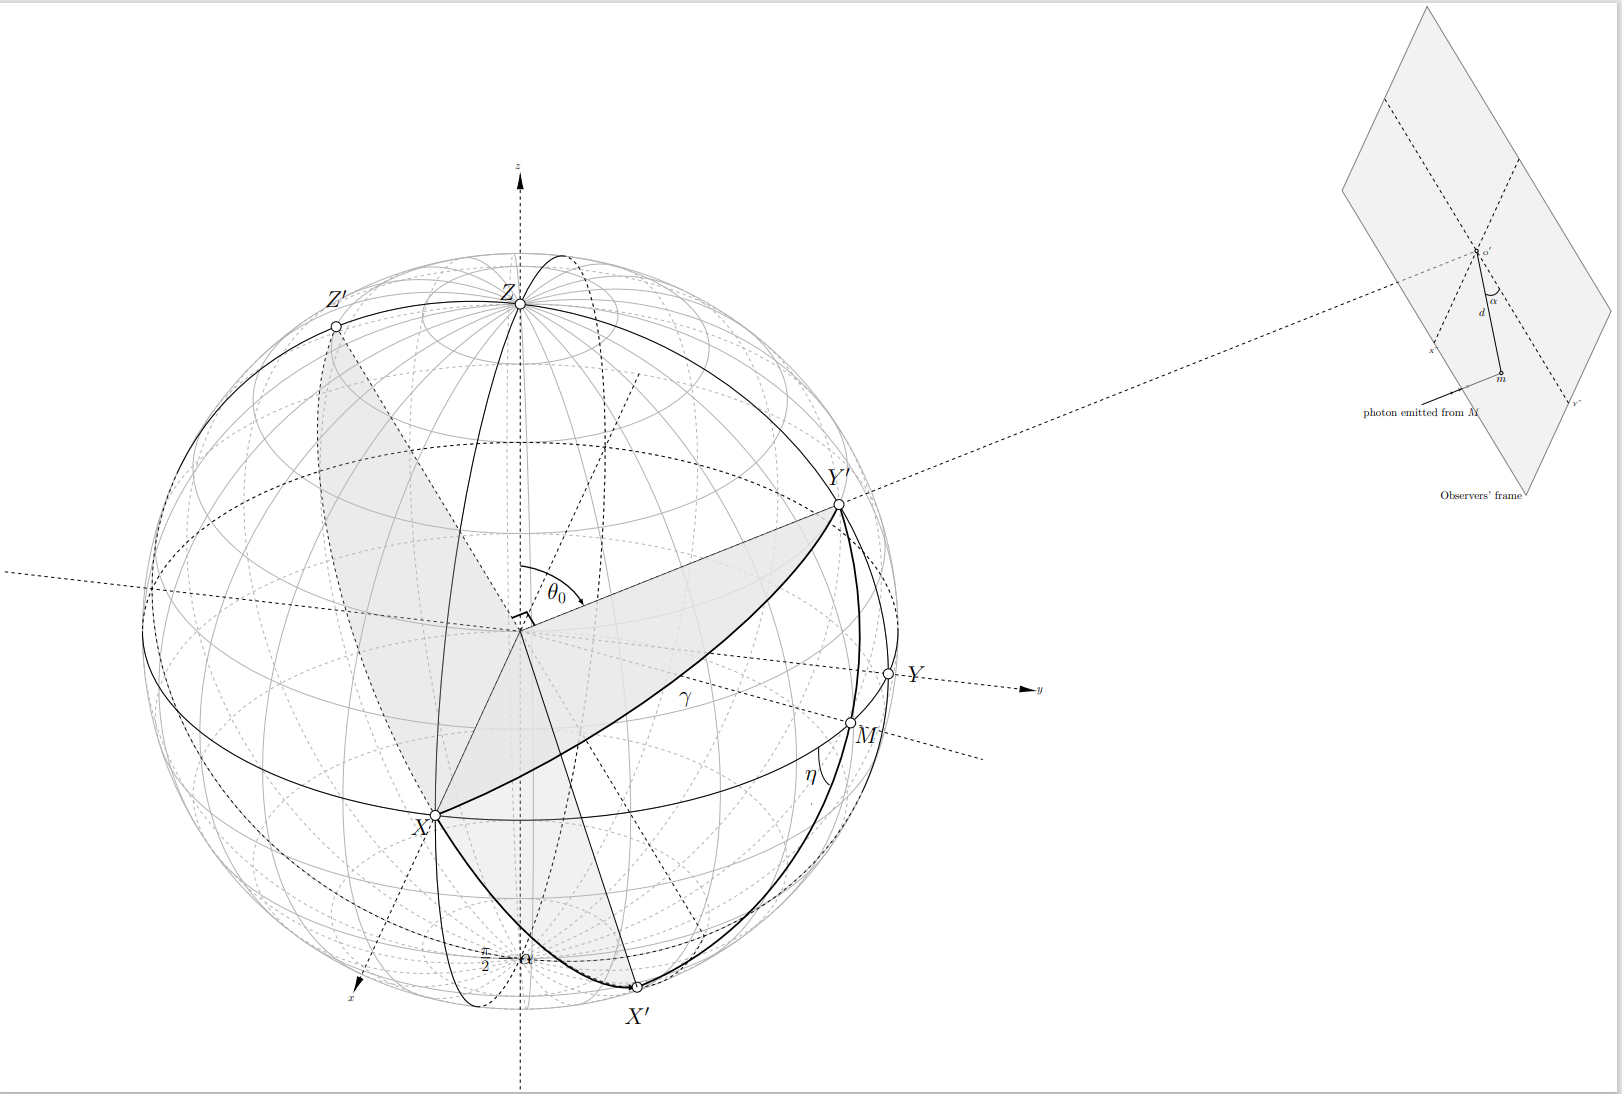
\includegraphics[width=15cm]{./images/coordinatesystem.PNG}
  %\caption{}
  \label{fig:test}
\end{figure}
\begin{comment}
\section*{Remarks and warnings}
You're welcome to use these notes, but they may contain errors, so proceed with caution : I graduated in 1979, went straight in the industry (where I didn't have to use fancy maths), and picked mathematics and physics again after I retired, so my mathematics got rusty  for sure. If you do find an error, typo's , I'd be happy to receive bug reports, suggestions, and the like, through Github.
\newpage
\end{comment}

\begin{comment}
\section*{References: I used following books}
\textbf{V. Frolov, A. Zelnikov}, \textit{Black Hole Physics}, 2011, Oxford University Press, Oxford\\
\textbf{J.L. Synge, A. Schild}, \textit{Tensor Calculus}, 1978, Dover Publications. New-York\\
\textbf{D. Beklémichev}, \textit{Cours de Géométrie analytique et d'Algèbre Linéaire}, 1988, Editions Mir-Moscou\\
\textbf{S.M. Selby (Ed.)}, \textit{CRC Standard Mathematical Tables $22^{nd}$ edition}, 1974, CRC Press, Cleveland \\
\end{comment}

\tableofcontents
\listoffigures
\chapter{3. Image of a clothed black hole}
\pagebreak[4]

\section{General setting}
\begin{figure}[H]
 \centering
\tdplotsetmaincoords{70}{93}

\begin{tikzpicture}[scale=1,tdplot_main_coords]
   
  % VARIABLES
  \def\R{2.5}
  \def\dist{12}
  \def\thetazero{60}
  \def\myphi{45}
    \def\thetazero{60}
   \def\myalpha{63.43495}
  \def\plate{3}
  \def\pie{3.1415}
  \def\k{5}
  \def\r{\R}
   \def\modulus#1#2{sqrt(\dist*\dist+#1*#1+#2*#2)}
    \def\teeta#1#2{atan(sqrt(#1*#1+#2*#2)/\dist)}
    \def\fee#1#2{acos(#1/sqrt(#1*#1+#2*#2))}
\def\factor{1.4}

%Initial setup: coordinates, black hole , ISCO, accretion disk,...
    \tdplotsetrotatedcoords{0}{0}{0};
 \tdplotsetcoord{O}{0}{0}{0};
  \tdplotsetrotatedcoords{0}{0}{0};
 \tdplotsetcoord{MM}{\R}{90}{\myphi};%point of photon emission
\tdplotsetcoord{MMM}{\R*1.9}{90}{\myphi};%azimuthal line  of photon emission
\tdplotsetcoord{MMMM}{-\R}{90}{\myphi};%azimuthal line  of photon emission
\tdplotsetcoord{MMMMM}{-\R*1.9}{90}{\myphi};%azimuthal line  of photon emission
 
 \tdplotsetrotatedcoords{-45}{39}{ 52.23};%Equatorial plane (Euler angles were computed using a Python code snippet
\begin{scope}[tdplot_rotated_coords]
 \def\coef{1.8};
\tdplotsetcoord{AZplane1}{sqrt(\coef*\coef*\R*\R+\dist*\dist)}{90}{atan(\dist/\R/\coef)};
\tdplotsetcoord{AZplane2}{sqrt(\coef*\coef*\R*\R+\dist*\dist)}{90}{180-atan(\dist/\R/\coef)};
\tdplotsetcoord{AZplane3}{-sqrt(\coef*\coef*\R*\R+\dist*\dist/4)}{90}{180-atan(\dist/\R/2/\coef)};
\tdplotsetcoord{AZplane4}{-sqrt(\coef*\coef*\R*\R+\dist*\dist/4)}{90}{atan(\dist/\R/2/\coef)};
 \draw[dashdotted,tdplot_main_coords](AZplane1)--(AZplane2)-- (AZplane4)--(AZplane3)--cycle;
 \node[right] at (AZplane3){$\text{Photon equatorial plane}$};
\end{scope}%end of equatorila plane
 
 
  
  % AXES
  \tdplotsetrotatedcoords{0}{0}{0};
   \tdplotsetcoord{Z1}{\factor*\R}{0}{90};%z-axis
   \tdplotsetcoord{X}{1.3*\factor*\R}{90}{0};%x-axis
   
  \fill[fill = lightgray!50] (0,0,0) circle (1.3*\R);%accretion disk
  \draw[dashed] (0,0,0) circle (\R);orbit of emmiting particle
  \fill[fill = white] (0,0,0) circle (\R/4);%ISCO
  \tdplotsetrotatedcoords{0}{90}{0};%change plane of drawing (Tikz stuff)
  \fill[fill = black,tdplot_rotated_coords] (0,0,0) circle (\R/10);%black hole
  \tdplotsetrotatedcoords{0}{0}{0};

  
  \node[left=70,right] at (0,-{\R},0){Accretion disk};
  
   \tdplotsetcoord{Z}{\factor*\R}{0}{0};
   \draw[tdplot_rotated_coords,very thick,-{Latex[length=3mm, width=1mm]}] (O) -- (Z1)node[right]{$z$};;
   % theta_0 angle
  \tdplotsetrotatedcoords{0}{90}{90} % set the rotated coordinate system
\tdplotdrawarc[tdplot_rotated_coords,very thick,,->]{(O)}{1}{90}{90-\thetazero}{anchor=south}{$\theta_0$} ;%arc z-axis->observation line
  
  %OBSERVER
\tdplotsetrotatedcoords{90}{\thetazero}{270} % set the rotated coordinate system
  \begin{scope}[tdplot_rotated_coords] % use the rotated coordinate system
   \tdplotsetcoord{Obs}{\dist}{0}{0)};
   %Let's travel to the observer
  \tdplotsetrotatedcoordsorigin{(Obs)};
  %Photographic Plate
 \draw[tdplot_rotated_coords,decoration={markings, 
mark= at position 0.70 with with {\arrowreversed[scale=2]{>}},
	mark= at position 0.5 with {\arrowreversed[scale=2]{>}},
	mark= at position 0.3 with {\arrowreversed[scale=2]{>}}},postaction={decorate}] ({sin(\myalpha)*\plate},{cos(\myalpha)*\plate},0)-- ({sin(\myalpha)*\plate},{cos(\myalpha)*\plate},-1)node[{anchor=south east},xshift=0.2cm] {$\begin{array}{c}
photon \,emitted \\
 from \,M
\end{array}$ };
 \draw[tdplot_rotated_coords,dashed] (O)--(Obs);
\draw[fill= gray!20,opacity=.5,tdplot_rotated_coords](\plate,\plate,0)-- (\plate,-\plate,0)--(-\plate,-\plate,0)-- (-\plate,\plate,0)--cycle;

\draw[tdplot_rotated_coords,dashed](0,\plate,0)-- (0,-\plate,0);
\draw[tdplot_rotated_coords,dashed](\plate,0,0)-- (-\plate,0,0);
\node[right=2,right] at (Obs) {\tiny$O^{'}$};


%\tdplotresetrotatedcoordsorigin
\tdplotsetcoord {Xaccc}{\modulus{\plate}{0}}{\teeta{\plate}{0}}{\fee{\plate}{0}};
\tdplotsetcoord  {Yaccc} {\modulus{0}{\plate}}{\teeta{0}{\plate}}{\fee{0}{\plate}};
\node[left] at (Xaccc) {\tiny$X^{"}$};
\node[right] at (Yaccc) {\tiny$Y^{"}$};
 \tdplotsetcoord{m}{\modulus{\plate}{\plate}}{0}{\myalpha};
\draw[tdplot_rotated_coords,ultra thick,](0,0,0)-- ({sin(\myalpha)*\plate},{cos(\myalpha)*\plate},0)node[right] {$m$ };
\tdplotdrawarc[tdplot_rotated_coords]{(Obs)}{\plate/2.5}{90}{90-\myalpha}{below,xshift=0.1cm }{$\alpha$}
\draw[tdplot_rotated_coords,](0,0,0)+({1.8*sin(\myalpha)*\plate/2},{1.5*cos(\myalpha)*\plate/2})node[left] {$d$ };;
\tdplotsetcoord{mphoton}{0.9*\modulus{\plate}{\plate}}{10.75}{90};
\draw[tdplot_rotated_coords,](0,0,0)+(-4.8*\plate/1,2.2*\plate/1,0)node[left] {$\begin{array}{c}
Observers' \\
frame
\end{array}$ };;
\draw[fill = lightgray!50] (Obs) circle (0.5pt);
\end{scope}
%Let's go back to the black hole



  % draw photon geodesic
 
\tdplotsetrotatedcoords{-45}{39}{ 52.23};
\begin{scope}[tdplot_rotated_coords]
 \draw[tdplot_rotated_coords, thick,dashed](\R,0,0) arc [start angle=0,end angle=90,x radius=\R,y radius=\R];;
 \draw[tdplot_rotated_coords,thick, dashed](0,\R,0) arc [start angle=90,end angle=270,x radius=\R,y radius=\R];
\draw[tdplot_rotated_coords,thick,dashed](\R,0,0) arc [start angle=0,end angle=-90,x radius=\R,y radius=\R];
\def\omega{1.8*180/3.14159}
\def\epsilon{0.18}
\def\a{\epsilon}
\draw[ultra thick,variable=\t,domain=pi/9:1.12*pi,samples=100] plot ({(\R+\a*(\t-pi/9))*cos(\t *\omega)},{(\R+\a*(\t-pi/9))*sin(\t *\omega)},{0});
\def\coef{1};
\tdplotsetcoord{AZphoton}{sqrt(\coef*\coef*\plate/2*\plate/2+\dist*\dist)}{90}{atan(\dist/\plate/2/\coef)};
\tdplotsetcoord{photon}{\R+\a*3.10669}{90}{3};%point where photon leaves the BH's influence
\draw[ultra thick] (photon)--(mphoton);
\end{scope}

%Final decorations
   \tdplotsetcoord{Yacc}{\R}{\thetazero}{90};
   \draw[fill = white, tdplot_rotated_coords] (Yacc) circle (1.5pt)node[right=0.2cm]{\large$Y’$};
\node[below=2,right,tdplot_rotated_coords,] at (MM) {\large$M$};
  \draw[ tdplot_main_coords,dashed] (O)--(MMM);
  \draw[ tdplot_main_coords,dashed] (O)--(MMMM);
   \draw[ tdplot_main_coords,dashed] (MMMMM)--(MMMM);
  \draw[fill = white,tdplot_rotated_coords,] (MM) circle (1.5pt);
 \draw[fill = white,tdplot_rotated_coords,] (MMMM) circle (1.5pt);
  
  %perpendicular slice  to observer
      \tdplotsetrotatedcoords{270}{-\thetazero}{0};
      \begin{scope}[tdplot_rotated_coords]
      \tdplotdrawarc[tdplot_rotated_coords,very thick,,->]{(MM)}{-3.5}{\myalpha+10}{\myalpha+18}{anchor = south west}{$\frac{\pi}{2}-\alpha$} ;
\end{scope}
\draw[->,dashed] (0,0,0)--(X)node[left]{$x$};
\end{tikzpicture}


\caption{General setting.}
\label{fig:fig_4}
\end{figure}
$$\blacklozenge$$\newpage
\section{The coordinate system (enhanced):}

\begin{figure}[H]
 \centering
\tikzset{>=latex} % for LaTeX arrow head
\tikzstyle{proj}=[projcol!80,line width=0.08] %very thin
\tikzstyle{area}=[draw=veccol,fill=veccol!80,fill opacity=0.6]
\tikzstyle{vector}=[-stealth,myblue,thick,line cap=round]
\tikzstyle{unit vector}=[->,veccol,thick,line cap=round]
\tikzstyle{dark unit vector}=[unit vector,veccol!70!black]
\tikzset{ra/.style={red,draw,angle radius=0.5cm}} % right angle style

   
% 3D AXIS with spherical coordinates
\def\aofv{103}
\tdplotsetmaincoords{60}{\aofv}
\begin{tikzpicture}[scale=3,tdplot_main_coords]
   
  % VARIABLE
  \def\R{4.0}
  \def\dist{12}
  \def\angle{60}
  \def\plate{2}
  \def\pie{3.1415}
  \def\k{5}
  \def\r{\R}
  \def\beta{atan(\plate/2/\dist)}
  \def\teta{atan(2*\plate/2/sqrt(2)/\k/\dist)}
    \def\fie{acos(1/sqrt(2))}
 \def\done{sqrt(\dist*\dist +\plate*\plate/4)}
  \def\dtwo{sqrt(\dist*\dist +\plate*\plate/2/\k/\k)}
   \def\modulus#1#2{sqrt(\dist*\dist+#1*#1+#2*#2)}
    \def\teeta#1#2{atan(sqrt(#1*#1+#2*#2)/\dist)}
    \def\fee#1#2{acos(#1/sqrt(#1*#1+#2*#2))}
\def\factor{1.4}
 \def\az{74}%point of emmited photon
  
  \contourlength{0.8pt}
  % Draw sphere
   \draw[tdplot_screen_coords,thin,black!30] (0,0,0) circle (\r);
    \foreach \a in {-75,-60,...,75}
      {\tdplotCsDrawLatCircle[thin,black!30]{\r}{\a}}
    \foreach \a in {0,15,...,165}
      {\tdplotCsDrawLonCircle[thin,black!30]{\r}{\a}}
      \tdplotCsDrawLonCircle[,black]{\R}{90};
       \tdplotCsDrawLonCircle[black]{\R}{180};
    	\tdplotCsDrawLatCircle  []{\r}{0};
       
  % AXES
  \tdplotsetrotatedcoords{0}{0}{0};
 \tdplotsetcoord{O}{0}{0}{0};
  \tdplotsetcoord{Y1}{\factor*\R}{90}{90};
   \tdplotsetcoord{Y2}{-\factor*\R}{90}{90};
     \tdplotsetcoord{X1}{1.4*\factor*\R}{90}{0};
   \tdplotsetcoord{X2}{-\factor*\R}{90}{0};
        \tdplotsetcoord{Z1}{\factor*\R}{0}{90};
   \tdplotsetcoord{Z2}{-\factor*\R}{0}{-90};
   \tdplotsetcoord{Z}{\factor*\R}{0}{0};
  \draw[tdplot_rotated_coords,dashed,-{Latex[length=5mm, width=2mm]}] (X2) -- (X1) node[left=2,below]{$x$};;
  \draw[tdplot_rotated_coords,dashed,-{Latex[length=5mm, width=2mm]}] (Y2) -- (Y1) node[left=2,right]{$y$};;
   \draw[tdplot_rotated_coords,dashed,-{Latex[length=5mm, width=2mm]}] (Z2) -- (Z1)node[left=2,above]{$z$};;
   % theta_0 angle
   \tdplotsetrotatedcoords{0}{90}{90} % set the rotated coordinate system
\tdplotdrawarc[tdplot_rotated_coords,very thick,,->]{(O)}{0.8}{90}{90-\angle}{anchor=north}{\huge$\theta_0$} 
               \coordinate(M2) at ({\factor*\R*cos(\az)}, {\factor*\R*sin(\az)},0) ;
         \draw[ tdplot_main_coords,dashed] (O)--(M2);
  %OBSERVER
\tdplotsetrotatedcoords{90}{\angle}{270} % set the rotated coordinate system
  \begin{scope}[tdplot_rotated_coords] % use the rotated coordinate system
   \tdplotsetcoord{Obs}{\dist}{0}{0)};

  
   %Let's travel to the observer
  \tdplotsetrotatedcoordsorigin{(Obs)};

  %Photographic Plate
 \draw[tdplot_rotated_coords,decoration={markings, 
mark= at position 0.60 with {\arrowreversed{stealth}},
	mark= at position 0.5 with {\arrowreversed{stealth}},
	mark= at position 0.4 with {\arrowreversed{stealth}}},postaction={decorate}](\plate/2,\plate/2,0)--(\plate/2,\plate/2,-1)node[below] {photon emitted from $M$ };;%\draw[tdplot_rotated_coords] (0,0,0) + (30:.5) node {\tiny$m$ };

 \draw[tdplot_rotated_coords,dashed] (O)--(Obs);
\draw[fill= gray!20,opacity=.5,tdplot_rotated_coords](\plate,\plate,0)-- (\plate,-\plate,0)--(-\plate,-\plate,0)-- (-\plate,\plate,0)--cycle;


\draw[tdplot_rotated_coords,dashed](0,\plate,0)-- (0,-\plate,0);
\draw[tdplot_rotated_coords,dashed](\plate,0,0)-- (-\plate,0,0);
\node[right=2,right] at (Obs) {\tiny$O^{'}$};

%Let's go back to the black hole
\tdplotresetrotatedcoordsorigin
\tdplotsetcoord {Xaccc}{\modulus{\plate}{0}}{\teeta{\plate}{0}}{\fee{\plate}{0}};
\tdplotsetcoord  {Yaccc} {\modulus{0}{\plate}}{\teeta{0}{\plate}}{\fee{0}{\plate}};
\node[below] at (Xaccc) {\tiny$X^{"}$};
\node[right] at (Yaccc) {\tiny$Y^{"}$};
 \tdplotsetcoord{m}{\modulus{\plate/2}{\plate/2}}{\teeta{\plate/2}{\plate/2}}{\fee{\plate/2}{\plate/2}};
%\node[tdplot_rotated_coords,right] at(m) {$m$ };
\draw[tdplot_rotated_coords,](0,0,0)-- (\plate/2,\plate/2,0)node[below] {$m$ };;
\tdplotdrawarc[tdplot_rotated_coords]{(Obs)}{\plate/4}{45}{90}{anchor=north}{$\alpha$}
\draw[tdplot_rotated_coords,](0,0,0)+(\plate/4,\plate/4,0)node[left] {$d$ };;
\draw[tdplot_rotated_coords,](0,0,0)+(\plate/1,\plate/1,0)node[left] {Observers' frame };;
\draw[fill = lightgray!50] (Obs) circle (0.5pt);
\draw[fill = lightgray!50] (m) circle (0.5pt);
\end{scope}

 %draw perpendicular slice  to observer
      \tdplotsetrotatedcoords{270}{-\angle}{0};
      \begin{scope}[tdplot_rotated_coords]
      \draw[tdplot_rotated_coords,dashed,](\R,0*\R,0) arc [start angle=0,end angle=180,x radius=\R,y radius=\R]--(0,0,0)--cycle;
\path[tdplot_rotated_coords, thin , fill=gray!50,opacity=.21](0,0,0)-- (\R,0*\R,0) arc [start angle=0,end angle=90+\angle,x radius=\R,y radius=\R]--(0,0,0)--cycle;
\path[tdplot_rotated_coords, thin ,fill=gray!50,opacity=.11](0,0,0)-- (\R,0*\R,0) arc [start angle=0,end angle=90,x radius=\R,y radius=\R]--(0,0,0)--cycle;

% pi/2-alpha  angle
 \draw[tdplot_rotated_coords,thick,->,ultra thick](0*\R,1*\R,0) arc [start angle=90,end angle=90+\angle,x radius=\R,y radius=\R]node[midway,anchor = north east]{\huge$\frac{\pi}{2}-\alpha$};
\end{scope}

%draw slice  along to observer
\tdplotsetrotatedcoords{270}{270-\angle}{0};
\begin{scope}[tdplot_rotated_coords]
\draw[tdplot_rotated_coords,thin](0,0,0)-- (\R,0*\R,0) arc [start angle=0,end angle=90,x radius=\R,y radius=\R]--(0,0,0)--cycle;
\path[tdplot_rotated_coords,thin,fill=gray!20,opacity=0.8](0,0,0)-- (\R,0*\R,0) arc [start angle=0,end angle=90,x radius=\R,y radius=\R]--(0,0,0)--cycle;
\draw[tdplot_rotated_coords,ultra thick] (\R,0*\R,0) arc [start angle=0,end angle=90,x radius=\R,y radius=\R]node[midway,below=0.5cm]{\huge$\gamma$};;

\end{scope}



  % draw geodesic
\begin{scope}[tdplot_main_coords]
        \tdplotdefinepoints(0,0,0)(0,\R*sin(\angle),\R*cos(\angle))(\R*0.5,\R*0.433,-0.75*\R)
        \tdplotdrawpolytopearc[ultra thick]{\R}{}{}
    \end{scope}
    
   %Point of emmitted photon
  
\coordinate(M) at ({\R*cos(\az)}, {\R*sin(\az)},0) ;

    

%Final decorations
\tdplotsetcoord{Xb}{\R}{90}{0};
   \draw[fill = white, tdplot_rotated_coords] (Xb) circle (1.5pt)node[{anchor=north east}]{\huge$X$};;
   \tdplotsetcoord{Yb}{\R}{90}{90};
   \draw[fill = white, tdplot_rotated_coords] (Yb) circle (1.5pt)node[right=0.5cm]{\huge$Y$};;
   \tdplotsetcoord{Zb}{\R}{0}{0};
   \draw[fill = white, tdplot_rotated_coords] (Zb) circle (1.5pt) node[{anchor=south east}]{\huge$Z$};;
   \tdplotsetcoord{Yacc}{\R}{\angle}{90};
   \draw[fill = white, tdplot_rotated_coords] (Yacc) circle (1.5pt)node[above=0.5cm]{\huge$Y’$};

    \draw[fill = white, tdplot_rotated_coords] (M) circle (1.5pt)node[{anchor = north west}]{\huge$M$};

    \draw[fill = white, tdplot_main_coords] (\R*0.5,\R*0.433,-0.75*\R) circle (1.5pt)node[below=0.5cm]{\huge$X'$};;
    \draw[fill = white, tdplot_main_coords] (O)--(\R*0.5,\R*0.433,-0.75*\R) ;
    \coordinate(Zacc) at (0,{-\R*cos(\angle)},{\R*sin(\angle)} );
    \draw[fill = white,  tdplot_main_coords] (Zacc) circle (1.5pt)node[above=0.5cm]{\huge$Z'$};
    \pic[draw = black,angle radius =0.5cm, ultra thick]{right angle= Yacc--O--Zacc};
     \coordinate(Nu) at ({1.16*\R*cos(\az*0.7}, {1.16*\R*sin(\az*0.75)},0) ;

     \draw[ tdplot_main_coords] (Nu)--(Nu)node[above=0.5cm]{\huge$\eta$};
 



\tdplotsetrotatedcoords{\az}{90}{270} % set the rotated coordinate system
  \begin{scope}[tdplot_rotated_coords] % use the rotated coordinate system
   \tdplotsetcoord{M1}{\R}{0}{0)};
  \tdplotsetrotatedcoordsorigin{(M1)};
\tdplotdrawarc[tdplot_rotated_coords,thick]{(M1)}{0.7}{-5}{49}{midway, left}{};
 \end{scope}
\end{tikzpicture}
\caption{The coordinate system (see text).}
\label{fig:fig_3}
\end{figure}
$$\blacklozenge$$\newpage



\section{Angles relationships: equations $(9)$ and $(10)$}

\begin{figure}[H]
 \centering
\tdplotsetmaincoords{70}{120}

\begin{tikzpicture}[scale=1,tdplot_main_coords]
   
  % VARIABLE
  \def\R{4.0}
  \def\thetazero{60}
  \def\myphi{45}
    \def\thetazero{60}
  \def\myalpha{63.43495}
 
  \def\r{\R}
 \def\az{74}
    \tdplotsetrotatedcoords{0}{0}{0};
     \begin{scope}[tdplot_rotated_coords]
 \tdplotsetcoord{O}{0}{0}{0};%origin
  \tdplotsetcoord{xaxis}{\R*1.4}{90}{0};%origin
   \tdplotsetcoord{yaxis}{\R*1.4}{90}{90};%origin
    \tdplotsetcoord{zaxis}{\R}{0}{0};%origin
    \draw[-{Latex[length=3mm, width=1mm]} ](O)--(xaxis);
      \draw[-{Latex[length=3mm, width=1mm]} ] (O)--(yaxis);
        \draw[-{Latex[length=3mm, width=1mm]} ] (O)--(zaxis);
 \tdplotsetcoord{MM}{\R}{90}{\myphi};%emmiting particle
  \tdplotsetcoord{Y}{\R}{90}{90};%y-axis
  \tdplotsetcoord{X}{\R}{90}{0};%x-axis
  \tdplotsetcoord{Yaccent}{\R}{\thetazero}{90};%observers axis
  \end{scope}
 \tdplotsetrotatedcoords{270}{90-\thetazero}{90};%The point X'.
 \begin{scope}[tdplot_rotated_coords] 
 \tdplotsetcoord{Xaccent}{\R}{90-\myalpha+90}{0};%the observers x-axis
 \end{scope}
  \tdplotsetrotatedcoords{0}{0}{0}
  \begin{scope}[tdplot_rotated_coords]%theX-Y arc
   \draw[tdplot_rotated_coords,thick,ultra thick](0,\R,0) arc [start angle=90,end angle=0,x radius=\R,y radius=\R];
\end{scope}
  \tdplotsetrotatedcoords{0}{90}{0}
  \begin{scope}[tdplot_rotated_coords]%the Y-Y' arc
  \draw[tdplot_rotated_coords,thick,ultra thick](0,\R,0) arc [start angle=90,end angle=90+90-\thetazero,x radius=\R,y radius=\R]node[midway,anchor = south west]{$\frac{\pi}{2}-\theta_0$};
\end{scope}
 \tdplotsetrotatedcoords{270}{-\thetazero}{0};
 \begin{scope}[tdplot_rotated_coords]%the X-X' arc
  \draw[tdplot_rotated_coords,thick,ultra thick](0,\R,0) arc [start angle=90,end angle=90+90-\myalpha,x radius=\R,y radius=\R]node[midway,anchor =north east]{$\frac{\pi}{2}-\alpha$};
\end{scope}
\tdplotsetrotatedcoords{-90}{90-\thetazero}{0};
 \begin{scope}[tdplot_rotated_coords]%the X-X' arc
  \draw[tdplot_rotated_coords,thick,ultra thick](0,\R,0) arc [start angle=90,end angle=180,x radius=\R,y radius=\R]node[midway,above=0.2cm]{$\frac{\pi}{2}$};
\end{scope}
  % draw geodesic
 \tdplotsetrotatedcoords{-45}{39}{ 52.23};
\begin{scope}[tdplot_rotated_coords]%the X'-Y' arc (the pothon path)
 \draw[tdplot_rotated_coords,ultra thick](\R,0,0) arc [start angle=0,end angle=90,x radius=\R,y radius=\R];%node[midway,anchor = south east]{\large$\mathbf{\gamma}$};;
\end{scope}

%Final decorations

 
\node[below,tdplot_rotated_coords,] at (MM) {$M$};
 \draw[dashed] (O)--(MM);
  \draw[dashed] (O)--(Yaccent);
  \draw[fill = white,tdplot_rotated_coords,] (MM) circle (1.5pt);
\tdplotsetrotatedcoords{0}{90}{270} % set the rotated coordinate system
 \tdplotdrawarc[tdplot_rotated_coords,thick]{(MM)}{-1.2}{19}{48}{anchor=south  west}{$\eta$};
 \tdplotdrawarc[tdplot_rotated_coords,thick]{(MM)}{1.2}{41}{12}{anchor=north  east}{$\eta$};;

\pic[draw = black,angle radius =0.25cm, ]{right angle= Yaccent--Y--MM};
\pic[draw = black,angle radius =0.25cm, ]{right angle=Yaccent--X--Xaccent};
\pic[draw = black,angle radius =0.25cm, ]{right angle=Yaccent--X--Xaccent};
\pic[draw = black,angle radius =0.25cm, ]{right angle=X--Yaccent--Y};
\pic[draw = black,angle radius =0.15cm, ]{right angle=Yaccent--Xaccent--X};

\node[above] at (X) {$X^{}$};
\node[below] at (Xaccent) {$X^{'}$};
\node[right] at (Y) {$Y^{}$};
\node[above] at (Yaccent) {$Y^{'}$};
\node[right=1.5cm] at (MM) {$\phi$};
\node[below= 0.75cm] at (O) {$\frac{\pi}{2}-\phi$};
\node[below left=0.8cm] at (MM) {$x^{}$};
\node[above left=0.9cm] at (Y) {$\gamma$};

\end{tikzpicture}
\caption{Different spheric triangles used to find a relation between $\phi,\, \theta_0,\, \alpha$.}
\label{fig:fig_5}
\end{figure}
Resolving the different spherical triangles in order to have a relation between $\phi,\, \theta_0,\, \alpha$.\\
We have (using the basis spherical triangles identities $\frac{\sin{a}}{\sin{A}}= \frac{\sin{b}}{\sin{B}}=\frac{\sin{c}}{\sin{B}}$ and $\cos{a}=\cos{b}\cos{c}+\sin{b}\sin{c}\cos{A}$)\\\\
i) $\Delta Y'_2MY$

\begin{align*}
\frac{\cos{\theta_0}}{\sin{\eta}}&=\frac{\sin{\gamma}}{\sin{\frac{\pi}{2}}}=\frac{\sin{\phi}}{\sin{Y_2}}\\
\cos{(\frac{\pi}{2}-\theta_0)}&=\cos{\gamma}\cos{\phi}+\sin{\gamma}\sin{\phi}\cos{\eta}\\
\cos{\gamma}&=\cos{(\frac{\pi}{2}-\theta_0)}\cos{\phi}+\sin{(\frac{\pi}{2}-\theta_0)}\sin{\phi}\cos{\frac{\pi}{2}}\\
\cos{\phi}&=\cos{\gamma}\cos{(\frac{\pi}{2}-\theta_0)}+\sin{\gamma}\sin{(\frac{\pi}{2}-\theta_0)}\cos{Y'_2}
\end{align*}
ii) $\Delta X'MX_2$
\begin{align*}
\frac{\cos{\alpha}}{\sin{\eta}}&=\frac{\sin{x}}{\sin{X_2}}=\frac{\cos{\phi}}{\sin{X^{'}}}\\
\cos{(\frac{\pi}{2}-\alpha)}&=\cos{(\frac{\pi}{2}-\phi)}\cos{x}+\sin{(\frac{\pi}{2}-\phi)}\sin{x}\cos{\eta}\\
\cos{(\frac{\pi}{2}-\phi)}&=\cos{(\frac{\pi}{2}-\alpha)}\cos{x}+\sin{(\frac{\pi}{2}-\alpha)}\sin{x}\cos{X'}\\
\cos{x}&=\cos{(\frac{\pi}{2}-\alpha)}\cos{(\frac{\pi}{2}-\phi)}+\sin{(\frac{\pi}{2}-\alpha)}\sin{(\frac{\pi}{2}-\phi)}\cos{X_1}
\end{align*}
iii) $\Delta YX_1X'$
\begin{align*}
\frac{\sin{\frac{\pi}{2}}}{\sin{\frac{\pi}{2}}}&=\frac{\cos{\theta_0}}{\sin{X_1}}=\frac{\sin{\frac{\pi}{2}}}{\sin{Y'}}\\
\cos{(\frac{\pi}{2}-\theta_0)}&=\cos{\frac{\pi}{2}}\cos{\frac{\pi}{2}}+\sin{\frac{\pi}{2}}\sin{\frac{\pi}{2}}\cos{X_1}\\
\cos{\frac{\pi}{2}}&=\cos{(\frac{\pi}{2}-\theta_0)}\cos{\frac{\pi}{2}}+\sin{(\frac{\pi}{2}-\theta_0)}\sin{\frac{\pi}{2}}\cos{\frac{\pi}{2}}\\
\cos{\frac{\pi}{2}}&=\cos{\frac{\pi}{2}}\cos{(\frac{\pi}{2}-\theta_0)}+\sin{\frac{\pi}{2}}\sin{(\frac{\pi}{2}-\theta_0)}\cos{Y'}
\end{align*}
iv) $\Delta XY'_1X'$
\begin{align*}
\frac{\cos{\alpha}}{\sin{Y'_1}}&=\frac{\sin{\frac{\pi}{2}}}{\sin{X'}}=\frac{\sin{(x+\gamma)}}{\sin{\frac{\pi}{2}}}\\
\cos{(\frac{\pi}{2}-\alpha)}&=\cos{\frac{\pi}{2}}\cos{(x+\gamma)}+\sin{\frac{\pi}{2}}\sin{(x+\gamma)}\cos{Y'_1}\\
\cos{\frac{\pi}{2}}&=\cos{(x+\gamma)}\cos{(\frac{\pi}{2}-\alpha)}+\sin{(x+\gamma)}\sin{(\frac{\pi}{2}-\alpha)}\cos{X'}\\
\cos{(x+\gamma)}&=\cos{\frac{\pi}{2}}\cos{(\frac{\pi}{2}-\alpha)}+\sin{\frac{\pi}{2}}\sin{(\frac{\pi}{2}-\alpha)}\cos{\frac{\pi}{2}}
\end{align*}
Simplifying:
\begin{align*}
\frac{\cos{\theta_0}}{\sin{\eta}}&=\sin{\gamma}=\frac{\sin{\phi}}{\sin{Y_2}}\\
\frac{\cos{\alpha}}{\sin{\eta}}&=\frac{\sin{x}}{\sin{X_2}}=\frac{\cos{\phi}}{\sin{X^{'}}}\\
\cos{\theta_0}&=\sin{X_1}\\
Y'&=\frac{\pi}{2}\\
\frac{\cos{\alpha}}{\sin{Y'_1}}&=\frac{1}{\sin{X'}}=\sin{(x+\gamma)}\\
\sin{\theta_0}&=\cos{\gamma}\cos{\phi}+\sin{\gamma}\sin{\phi}\cos{\eta}\\
\cos{\gamma}&=\sin{\theta_0}\cos{\phi}\\
\cos{\phi}&=\cos{\gamma}\sin{\theta_0}+\sin{\gamma}\cos{\theta_0}\cos{Y'_2}\\
\sin{\alpha}&=\sin{\phi}\cos{x}+\cos{\phi}\sin{x}\cos{\eta}\\
\sin{\phi}&=\sin{\alpha}\cos{x}+\cos{\alpha}\sin{x}\cos{X'}\\
\cos{x}&=\sin{\alpha}\sin{\phi}+\cos{\alpha}\cos{\phi}\cos{X_1}\\
\sin{\theta_0}&=\cos{X_1}\\
\sin{\alpha}&=\sin{(x+\gamma)}\cos{Y'_1}\\
0&=\cos{(x+\gamma)}\sin{\alpha}+\sin{(x+\gamma)}\cos{\alpha}\cos{X'}\\
0&=\cos{(x+\gamma)}
\end{align*}
and get (discarding all other equation which are not relevant for the problem):
\begin{align}
\frac{\cos{\theta_0}}{\sin{\eta}}&=\sin{\gamma}\\
\frac{\cos{\alpha}}{\sin{\eta}}&=\cos{\phi}\\
\cos{\gamma}&=\sin{\theta_0}\cos{\phi}
\end{align}
From $(1)$ and $(2)$ we get \footnote{In the paper, in equation $(9)$ we see $\cos{\alpha}= \frac{\cot{\phi}\cos{\theta_0}}{\sin{\gamma}}$, which is wrong ($\cot{\phi}$ should be $\cos{\phi})$ as otherwise $\cos{\alpha}$ could become greater than $1$ for certain values of $\phi$.}
\begin{align}\sin{\gamma} =\frac{\cos{\phi}\cos{\theta_0}}{\cos{\alpha}}\end{align} and combining this with $(3)$ we get (squaring both equations and  add them up)
$$\cos{\alpha}= \frac{\cos{\phi}\cos{\theta_0}}{\sqrt{1-\sin^2{\theta_0}\cos^2{\phi}}}$$\\
Equation $(10)$ in the paper follows from equations $(3)$ and $(4)$ by elimination of $\phi$.

$$\blacklozenge$$\newpage
\section{Derivation of equation $(11)$,  $(12)$, $(13)$.}
As can be seen in figure $3.2.$ the photon will reach the plaque (at infinity) after having spanned the angle $\gamma$. Hence,
\begin{align}
\gamma&= \frac{1}{\sqrt{2M}}\int_{0}^{\frac{1}{r}}\frac{dt}{\sqrt{G(t)}}\nonumber \\
&= \underbrace{\frac{1}{\sqrt{2M}}\int_{0}^{\frac{1}{P}}\frac{dt}{\sqrt{G(t)}}}_{2\sqrt{\frac{P}{Q}}\left[K{\left(k\right)}-F{\left(\zeta_{\infty},k\right)}\right]}+\frac{1}{\sqrt{2M}}\int_{\frac{1}{P}}^{\frac{1}{r}}\frac{dt}{\sqrt{G(t)}}\nonumber \\
&=2\sqrt{\frac{P}{Q}}\left[K{\left(k\right)}-F{\left(\zeta_{\infty},k\right)}\right]-\frac{1}{\sqrt{2M}}\int^{\frac{1}{P}}_{\frac{1}{r}}\frac{dt}{\sqrt{G(t)}}
\end{align}
Let's recall equation $(3)$ in section $2.3.$:
\begin{align}
E(z)
&=2\sqrt{2M}\sqrt{\frac{P}{Q}}\int_{\varphi}^{\frac{\pi}{2}}\frac{d\tau}{\sqrt{1-k^{2}\sin^{2}{\left(\tau\right)}}}\quad\quad\small{\left(x=\sin{\left(\tau\right)}\right)}
\end{align}
The upper integration limit $\frac{\pi}{2}$ corresponds to the $\frac{1}{P}$ spherical radial distance, but here for calculating  $\varphi=\arcsin{\left(\sqrt{\frac{z-u_1}{u_2-u_1}}\right)}\in\left(0,\frac{\pi}{2}\right)$ instead of taking $z=0$ as we did previously, we have to take $z=\frac{1}{r}$ which gives 
\begin{align}
\sin^2{\varphi}_{|z=\frac{1}{r}}&=\frac{\frac{1}{r}-u_1}{u_2-u_1}\nonumber \\
&=\frac{\frac{1}{r}+\frac{Q-P+2M}{4MP}}{\frac{1}{P}+\frac{Q-P+2M}{4MP}}\nonumber \\
&=\frac{Q-P+2M+\frac{4MP}{r}}{Q-P+6M}
\end{align}
Let's put \begin{align}\sin^2{\zeta_{r}}=\frac{Q-P+2M+\frac{4MP}{r}}{Q-P+6M}\end{align}\\
$(2)$ becomes
\begin{align}
E(z)
&=2\sqrt{2M}\sqrt{\frac{P}{Q}}\int_{\zeta_{r}}^{\frac{\pi}{2}}\frac{d\tau}{\sqrt{1-k^{2}\sin^{2}{\left(\tau\right)}}}\nonumber \\
&= 2\sqrt{2M}\sqrt{\frac{P}{Q}}\int_{\zeta_{r}}^{0}\frac{d\tau}{\sqrt{1-k^{2}\sin^{2}{\left(\tau\right)}}}+2\sqrt{2M}\sqrt{\frac{P}{Q}}\int_{0}^{\frac{\pi}{2}}\frac{d\tau}{\sqrt{1-k^{2}\sin^{2}{\left(\tau\right)}}}\nonumber \\
&= -2\sqrt{2M}\sqrt{\frac{P}{Q}}\int^{\zeta_{r}}_{0}\frac{d\tau}{\sqrt{1-k^{2}\sin^{2}{\left(\tau\right)}}}+2\sqrt{2M}\sqrt{\frac{P}{Q}}K{\left(k\right)}\nonumber \\
&= -2\sqrt{2M}\sqrt{\frac{P}{Q}}F{\left(\zeta_{r},k\right)}+2\sqrt{2M}\sqrt{\frac{P}{Q}}K{\left(k\right)}
\end{align}
Substituting this in $(1)$:
\begin{align}
\gamma&=2\sqrt{\frac{P}{Q}}\left[K{\left(k\right)}-F{\left(\zeta_{\infty},k\right)}\right]-\frac{1}{\sqrt{2M}}2\sqrt{2M}\sqrt{\frac{P}{Q}}K{\left(k\right)}+\frac{1}{\sqrt{2M}}2\sqrt{2M}\sqrt{\frac{P}{Q}}F{\left(\zeta_{r},k\right)}\nonumber \\
&=2\sqrt{\frac{P}{Q}}\left[K{\left(k\right)}-F{\left(\zeta_{\infty},k\right)}\right]-2\sqrt{\frac{P}{Q}}K{\left(k\right)}+2\sqrt{\frac{P}{Q}}F{\left(\zeta_{r},k\right)}\nonumber \\
&= 2\sqrt{\frac{P}{Q}}\left[F{\left(\zeta_{r},k\right)} -F{\left(\zeta_{\infty},k\right)}\right]
\end{align}
The only term which depends explicitly on $r$ is $F{\left(\zeta_{r},k\right)}$. We rewrite $(5)$ as 
\begin{align}
F{\left(\zeta_{r},k\right)} &= \half \gamma\sqrt{\frac{Q}{P}}+F{\left(\zeta_{\infty},k\right)}
\end{align}

Let $\mathrm{sn}(u,k)$ be the usual Jacobian elliptic function with $ \sin{\zeta_{r}}= \mathrm{sn}(F{\left(\zeta_{r},k\right)})$.\\
We get
\begin{align*}
\sin{\zeta_{r}} &=\mathrm{sn}\left( \half \gamma\sqrt{\frac{Q}{P}}+F{\left(\zeta_{\infty},k\right)}\right)
\end{align*}
From which:
\begin{align}
&\sin^2{\zeta_{r}} =\mathrm{sn}^2\left( \half \gamma\sqrt{\frac{Q}{P}}+F{\left(\zeta_{\infty},k\right)}\right)\nonumber \\
(4)\,\implies\quad &\frac{Q-P+2M+\frac{4MP}{r}}{Q-P+6M} =\mathrm{sn}^2\left( \half \gamma\sqrt{\frac{Q}{P}}+F{\left(\zeta_{\infty},k\right)}\right)\nonumber \\
\implies\quad &\frac{1}{r} =-\frac{Q-P+2M}{4MP}+\frac{Q-P+6M}{4MP}\mathrm{sn}^2\left( \half \gamma\sqrt{\frac{Q}{P}}+F{\left(\zeta_{\infty},k\right)}\right)
\end{align}
Note that in the paper the coefficient $\frac{Q}{P}$ is wrongly written  as $\frac{P}{Q}$
$$\blacklozenge$$\newpage

The derivative of the Jacobi elliptic function $\text{sn}(u, k)$ with respect to the parameter $k$ is given by:

$$
\frac{d}{dk} \text{sn}(u, k) = \text{cn}(u, k) \, \text{dn}(u, k)
$$

Where $\text{cn}(u, k)$ and $\text{dn}(u, k)$ are the Jacobi elliptic functions associated with $\text{sn}(u, k)$.

The derivative of the Jacobi elliptic function $\text{sn}(u, k)$ with respect to the variable $u$ is given by:

$$
\frac{d}{du} \text{sn}(u, k) = \text{cn}(u, k) \, \text{dn}(u, k)
$$

Where $\text{cn}(u, k)$ and $\text{dn}(u, k)$ are the Jacobi elliptic functions associated with $\text{sn}(u, k)$.

The complete elliptic integral of the first kind, denoted as $K(k)$, is a function of the modulus $k$. Since it's not dependent on the variable $u$, its derivative with respect to $u$ is zero:

$$
\frac{d}{du} K(k) = 0
$$

The derivative of the complete elliptic integral of the first kind, $( K(k) )$, with respect to the parameter $( k )$ is given by:

$$[ \frac{dK(k)}{dk} = \frac{E(k)}{k(1-k^2)} ]$$

Where $( E(k) )$ is the complete elliptic integral of the second kind.


The derivative of the incomplete elliptic integral of the first kind, $( F(p, k) )$, with respect to the parameter $( k )$ is not expressible in simple elementary functions. However, it can be represented in terms of the elliptic integrals of the first and second kind and the complete elliptic integral of the first kind.

The derivative is given by:

$$[ \frac{dF(p, k)}{dk} = \frac{\Pi(n, k) - K(k)}{2k(1-k^2)} ]$$

Where $ ( n = 1 - p ), ( K(k) )$ is the complete elliptic integral of the first kind, and $( \Pi(n, k) )$ is the complete elliptic integral of the third kind with modulus $( n )$.

The derivative of the incomplete elliptic integral of the first kind, $( F(p, k) )$, with respect to the parameter $( p )$ is not expressible in simple elementary functions. However, it can be represented in terms of the elliptic integrals of the first and second kind and the complete elliptic integral of the first kind.

The derivative is given by:

$$[ \frac{dF(p, k)}{dp} = \frac{K(k') - E(k')}{2p(1-p)(1-k^2)} ]$$

Where $( k' = \sqrt{1 - k^2} )$,$ ( K(k) )$ is the complete elliptic integral of the first kind, and $( E(k) )$ is the complete elliptic integral of the second kind.
\end{document}